% !TeX root = proyecto.tex

%=========================================================
\chapter{Modelo del Negocio}	
\label{cap:reqSist}

\cdtInstrucciones{Introduzca el capítulo describiendo el contenido del mismo, su organización y propósito.}

%----------------------------------------------------------
\section{Actores del sistema}

	\cdtInstrucciones{En esta sección describa a los actores del sistema.}
	
	%---------------------------------------------------------
	\begin{Usuario}{\hypertarget{Cliente}{\subsection{Cliente}}}{
			Es todo aquel actor que no pertenezca a la empresa y que desea desea reservar, hospedar y contratar los servicios que ofrece la empresa para su mascota.
		}
		\item[Responsabilidades:] \cdtEmpty
		\begin{itemize}
			\item Brindar datos precisos y actualizados de identificación de su persona y de su(s) mascota(s) para registrarse en el sistema y contratar los servicios que ofrece la empresa.
			\item Gestionar sus mascotas registradas en el sistema.
			\item Brindar datos precisos y actualizados de los medicamentos y vacunas administradas a su(s) mascota(s).
			\item Brindar datos actualizados de las noches, cuartos y servicios que desea reservar, así como las fechas de llegada (check-in) y salida (check-out) del hotel.
			\item Brindar datos precisos, actualizados y necesarios para pagar en el sistema por los servicios que se adquieran.
		\end{itemize}
		
		\item[Perfil:] \cdtEmpty
		\begin{itemize}
			\item Público mexicano que disponga de los recursos para cubrir el hospedaje de sus mascotas.
			\item Posée una o más mascotas a las que la empresa pueda ofrecer sus servicios.
		\end{itemize}
		\item[Procesos en los que participa:] \cdtEmpty
		\begin{itemize}
			%TODO: Agregar los procesos en los que se involucrará al cliente
			\item .
		\end{itemize}
	\end{Usuario}

	
%---------------------------------------------------------
\section{Términos del Negocio}
\label{sec:terminosDeNegocio}

\cdtInstrucciones{En esta sección describa todos los términos del negocio que aparecen en la especificación del sistema.}
	
\begin{description}
	% Ejemplo de un término literal.
	\item[\hypertarget{tAutomovil}{Automóvil:}] ({\em es un tipo de \hyperlink{tVehiculo}{Vehículo}}) De cuatro ruedas con capacidad de 5 a 9 personas. 
	% Ejemplo de un término de entidad
	\item[\hypertarget{tCliente}{Cliente:}] Se refiere a todas las personas físicas y morales que \hyperlink{tRenta}{rentan} o han rentado un \hyperlink{tVehiculo}{vehículo}.
	
	\item[\hypertarget{tDirector}{Director:}] ({\em es un tipo de \hyperlink{tEmpleado}{Empleado}}) Es el empleado que tiene mayor rango de todos y no tiene superior, a diferencia de los demás.	
	\item[\hypertarget{tEmpleado}{Empleado:}] Se refiere a cualquier persona que labore en la empresa.
	
	\item[\hypertarget{tChecador}{Checador:}] ({\em Reloj asociado al atributo:} Hora de entrada y salida de un \hyperlink{tEmpleado}{empleado}. {\em Frecuencia de lectura:} Una vez al día para la entrada y otra para la salida durante los días laborales.
	
	\item[\hypertarget{tMotocicleta}{Motocicleta:}] ({\em es un tipo de {tVehiculo}{Vehículo}}) De dos ruedas con capacidad para una personas. 

	\item[\hypertarget{tRenta}{Renta:}] Se refiere al servicio que ofrece la empresa para prestar \hyperlink{tVehiculo}{vehículos} a los \hyperlink{tCliente}{clientes} por un tiempo definido.
	
	\item[\hypertarget{tVehiculo}{Vehiculo:}] Se refiere a los automóviles y motocicletas que la empresa usa para dar el servicio de renta a los \hyperlink{tCliente}{clientes}.
	
%	\brTermSensor{tVelocimetro}{Velocímetro:}{Velocidad de un Vehículo.}{Kilometros/hora.}{Constantemente siempre que el \cdtRef{tVehiculo}{vehículo} esté encendido.}
\end{description}

%----------------------------------------------------------
\section{Modelo del dominio del problema}
\label{sec:hechosDeNegocio}

\cdtInstrucciones{En esta sección describa todas las entidades del negocio y sus relaciones.}

	El modelo del dominio del problema se muestra en la figura~\ref{fig:modeloDeDominio}, a continuación se describen cada una de las entidades y sus relaciones.
	
\begin{figure}[htpb!]
	\begin{center}
		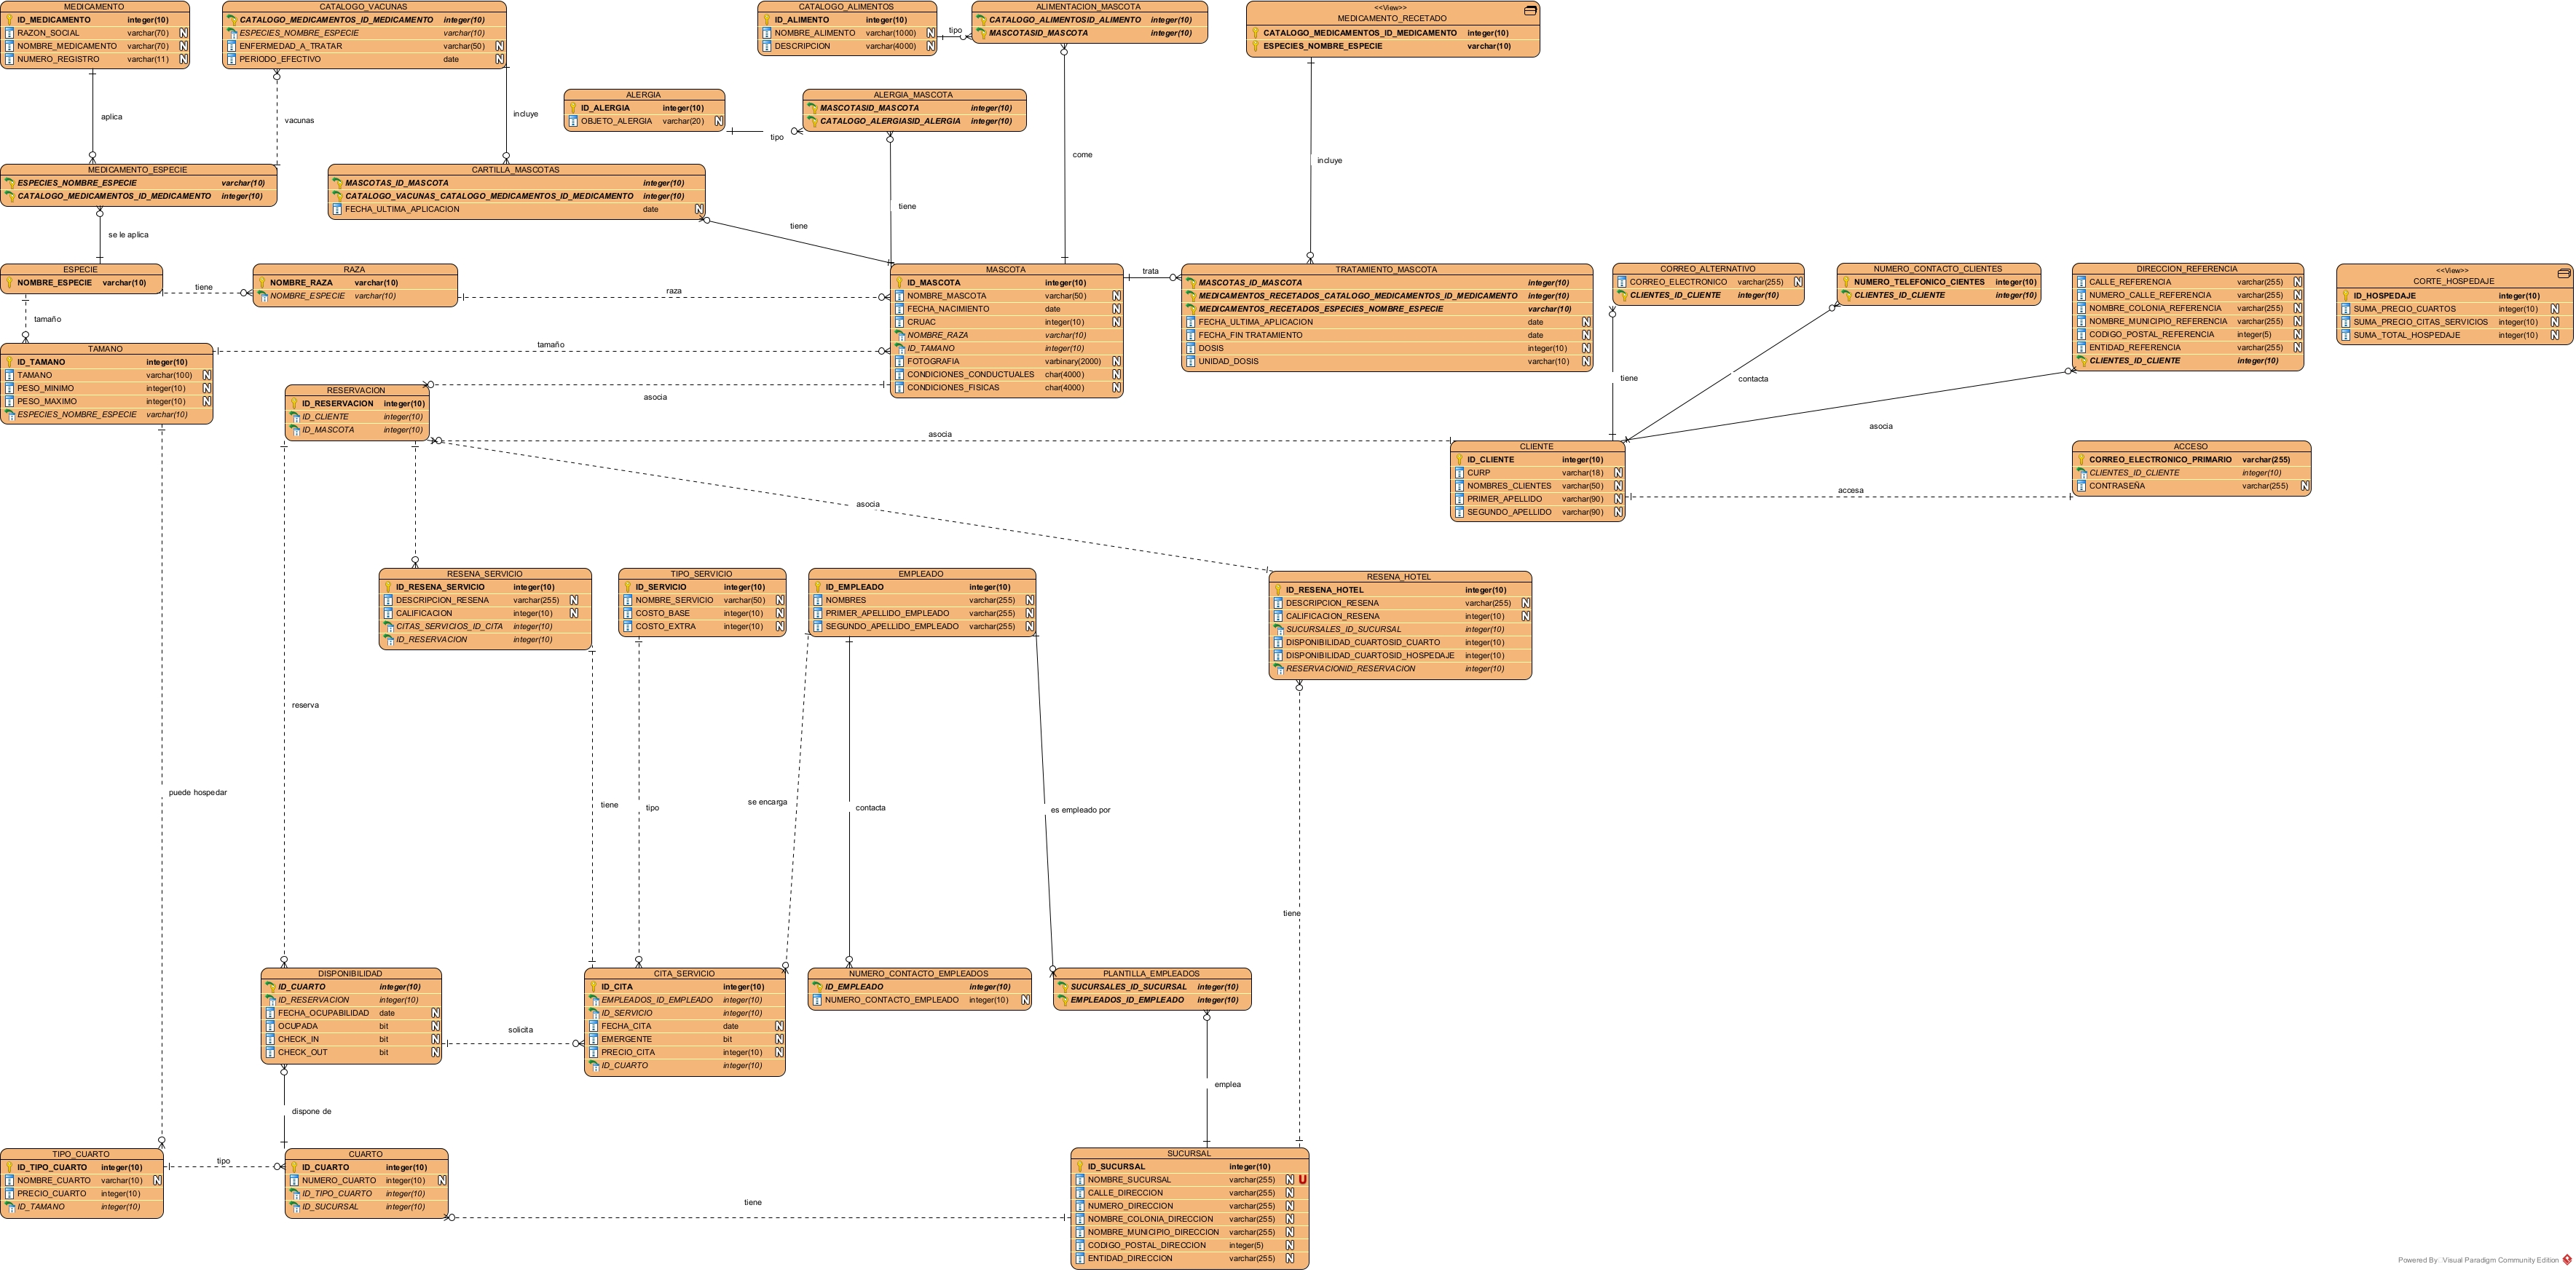
\includegraphics[angle=90,width=.60\textwidth]{images/Base_Datos}
		\caption{Modelo del dominio del problema}
		\label{fig:modeloDeDominio}
	\end{center}
\end{figure}

%\brRelComposition	Relación de composición
%\brRelAgregation	Relación de agregación
%\brRelGeneralization	Relación de generalización
%\brRelParticipation	Relación de participación
%- - - - - - - - - - - - - - - - - - - - - - - - - - - - - 
\begin{cdtEntidad}{mascota}{Mascota}%{}
	\brAttr{nombre}{Nombre}{Palabra Corta}
		{Nombre o nombres de la mascota.}{Sí}
	\brAttr{tamano}{Tamaño}{\hyperlink{tamanoMascota}{Tamaño mascota}}
		{Tamaño de la mascota.}{Sí}
	\brAttr{fechaNacimiento}{Fecha de Nacimiento}{date}
		{Fecha de nacimiento de la mascota.}{Sí}
	\brAttr{CRUAC}{CRUAC}{CURP}
		{CRUAC de la mascota.}{Sí}
	\brAttr{especie}{Especie}{\hyperlink{nombreEspecie}{Nombre especie}}
		{Especie de la mascota.}{Sí}
	\brAttr{raza}{Raza}{\hyperlink{nombreRaza}{Nombre raza}}
		{Raza de la mascota.}{Sí}
	\brAttr{foto}{Fotografia}{imagen}
		{Fotografia de la mascota.}{Sí}
	\brAttr{tipoVacuna}{Tipo de vacuna}{\hyperlink{vacunaMascota}{Vacuna mascota}}
		{Tipo de vacuna con la que cuenta la mascota.}{Sí}
	\brAttr{nombreVacuna}{Nombre de la vacuna}{Palabra corta}
		{Nombre de la vacuna con la que cuenta la mascota.}{Sí}
	\brAttr{fechaAplicacion}{Ultima fecha de aplicación}{date}
		{Ultima fecha de aplicación de la vacuna con la que cuenta la mascota.}{Sí}
	\brAttr{dosis}{Numero de dosis aplicadas}{Numero}
		{Numero de dosis aplicadas de la vacuna con la que cuenta la mascota.}{Sí}
	\brAttr{alergias}{Alergias}{\hyperlink{AlergiaMascota}{Alergia Mascota}}
		{Numero de dosis aplicadas de la vacuna con la que cuenta la mascota.}{Sí}
	\brAttr{tratamientoMedico}{Tratamiento Medico}{\hyperlink{tratamientoMedicoMascota}{Tratamiento medico mascota}}
		{Numero de dosis aplicadas de la vacuna con la que cuenta la mascota.}{Sí}
	\brAttr{caracteristicasEspeciales}{Caracteristicas Especiales}{varchar}
		{Caracteristicas especiales fisicas o de comportamiento de la mascota.}{Sí}
	%\cdtEntityRelSection
	%\brRel{\brRelAgregation}{País}{Un \hyperlink{Alumno}{Alumno} es originario de un \hyperlink{Pais}{Pais}}	
	%\brRel{\brRelGeneralization}{Alumno}{Un \hyperlink{AlumnoExtranjero}{Alumno Extranjero} es un  \hyperlink{Alumno}{Alumno}}	
	%\brRel{\brRelParticipation}{Alumno}{Un \hyperlink{AlumnoExtranjero}{Alumno Extranjero} es un  \hyperlink{Alumno}{Alumno}}	
\end{cdtEntidad}

\begin{cdtEntidad}{SUCURSAL}{Sucursal}
	\brAttr{ID_SUCURSAL}{ID de la sucursal}{ID}{ID interno asignado a cada sucursal.}{Sí}
	\brAttr{NOMBRE_SUCURSAL}{Nombre de la sucursal}{Cadena}{Nombre comercial de la sucursal.}{Sí}
	\brAttr{CALLE_DIRECCION}{Nombre de calle}{Cadena}{Calle de la dirección de la sucursal.}{Sí}
	\brAttr{NUMERO_DIRECCION}{Número de calle}{Cadena corta}{Número de calle de la dirección de la sucursal.}{Sí}
	\brAttr{NOMBRE_COLONIA_DIRECCION}{Nombre de colonia}{Frase corta}{Nombre de la colonia donde se ubica la sucursal.}{Sí}
	\brAttr{NOMBRE_MUNICIPIO_DIRECCION}{Nombre de municipio}{Frase corta}{Nombre del municipio donde se encuentra la sucursal.}{Sí}
	\brAttr{CODIGO_POSTAL_DIRECCION}{Código postal}{Numérico}{Código postal de la sucursal.}{Sí}
	\brAttr{ENTIDAD_DIRECCION}{Nombre de entidad}{Frase corta}{Entidad o estado donde se encuentra la sucursal.}{Sí}
	\cdtEntityRelSection
	\brRel{\brRelComposition}{Cuarto}{Una \hyperlink{SUCURSAL}{sucursal} tiene uno o más \hyperlink{CUARTO}{cuartos} en los que puede hospedar las mascotas de sus clientes.}
	\brRel{\brRelAgregation}{Empleado}{Una \hyperlink{SUCURSAL}{sucursal} tiene uno o más \hyperlink{EMPLEADO}{empleados} que trabajan en ella.}
	\brRel{\brRelComposition}{Reseña del hotel}{Una \hyperlink{SUCURSAL}{sucursal} tiene uno o más \hyperlink{RESENA_HOTEL}{reseñas} que califican sus estancias.}
\end{cdtEntidad}
%- - - - - - - - - - - - - - - - - - - - - - - - - - - - - 
\begin{cdtEntidad}{MEDICAMENTO}{Medicamento}
	\brAttr{ID_MEDICAMENTO}{ID del medicamento}{ID}{ID interno del medicamento de uso veterinario registrado en catálogos oficiales.}{Sí}
	\brAttr{RAZON_SOCIAL}{Razón social}{Frase}{Razón social de la empresa que desarrolló y produce el medicamento.}{Sí}
	\brAttr{NOMBRE_MEDICAMENTO}{Nombre del medicamento}{Frase}{Nombre comercial del medicamento.}{Sí}
	\brAttr{NUMERO_REGISTRO}{Número de registro}{ID}{Número de registro del medicamento en catálogos oficiales.}{Sí}
	\cdtEntityRelSection
	\brRel{\brRelComposition}{Especie}{Un \hyperlink{MEDICAMENTO}{medicamento} tiene una o más \hyperlink{ESPECIE}{especies} en las que se puede aplicar.}
\end{cdtEntidad}

%- - - - - - - - - - - - - - - - - - - - - - - - - - - - - 
\begin{cdtEntidad}{ESPECIE}{Especie}
	\brAttr{NOMBRE_ESPECIE}{Nombre de la especie}{Cadena}{Nombre de la especie de las mascotas.}{Sí}
	\cdtEntityRelSection
	\brRel{\brRelComposition}{Medicamento}{Una \hyperlink{ESPECIE}{especie} puede o no tener uno o más \hyperlink{MEDICAMENTO}{medicamentos} que se le pueden aplicar.}
	\brRel{\brRelGeneralization}{Raza}{Una \hyperlink{ESPECIE}{especie} tiene una o más \hyperlink{RAZA}{razas}.}
	\brRel{\brRelGeneralization}{Tamaño}{Una \hyperlink{ESPECIE}{especie} tiene uno o más \hyperlink{TAMANO}{tamaños}.}
	\brRel{\brRelAgregation}{Tipo de cuarto}{Un \hyperlink{TAMANO}{tamaño} de mascota puede o no tener uno o más \hyperlink{TIPO_CUARTO}{tipos de cuarto} en los que se puede hospedar.}
\end{cdtEntidad}

%- - - - - - - - - - - - - - - - - - - - - - - - - - - - - 
\begin{cdtEntidad}{RAZA}{Raza}
	\brAttr{NOMBRE_RAZA}{Nombre de la raza}{Cadena}{Nombre de la raza de las mascotas.}{Sí}
	\brAttr{NOMBRE_ESPECIE}{Nombre de la especie}{Palabra corta}{Nombre de la especie a la que pertenece la raza.}{Sí}
	\cdtEntityRelSection
	\brRel{\brRelComposition}{Mascota}{Una \hyperlink{ESPECIE}{raza} está asociado a una o más \hyperlink{MASCOTA}{mascotas}.}
\end{cdtEntidad}

%- - - - - - - - - - - - - - - - - - - - - - - - - - - - - 
\begin{cdtEntidad}{DISPONIBILIDAD_CUARTOS}{Disponibilidad de cuartos}
	\brAttr{ID_CUARTO}{ID del cuarto}{ID}{ID interno del cuarto en le que reservan.}{Sí}
	\brAttr{ID_HOSPEDAJE}{ID del hospedaje}{ID}{ID interno del hospedaje o estancia.}{No}
	\brAttr{ID_RESERVACION}{ID de reservación}{ID}{ID interno de la reservación que le corresponde a la estancia.}{Sí}
	\brAttr{FECHA_OCUPABILIDAD}{Fecha}{Fecha}{Fecha de disponibilidad.}{Sí}
	\brAttr{OCUPADA}{Ocupabilidad}{Booleano}{Indica si el cuarto está ocupado.}{Sí}
	\brAttr{CHECK-IN}{Check-in}{Booleano}{Indica si la fecha es el check-in.}{Sí}
	\brAttr{CHECK-OUT}{Check-out}{Booleano}{Indica si la fecha es el check-out.}{Sí}
	\brAttr{CHECK-IN}{Check-in}{Booleano}{Indica si el cuarto está ocupado.}{Sí}
	\cdtEntityRelSection
	\brRel{\brRelParticipation}{Reseña de servicio}{Un \hyperlink{TIPO_CUARTO}{tipo de cuarto} puede estar asociado a uno o más
\hyperlink{CUARTO}{cuartos}.}
\end{cdtEntidad}

%- - - - - - - - - - - - - - - - - - - - - - - - - - - - - 
\begin{cdtEntidad}{TIPO_CUARTO}{Tipo de cuarto}
	\brAttr{ID_TIPO_CUARTO}{ID del tipo de cuarto}{ID}{ID interno del tipo de cuarto que tienen todos los hoteles.}{Sí}
	\brAttr{NOMBRE_CUARTO}{Nombre del cuarto}{Frase corta}{Nombre comercial del tipo de cuarto del que dispone el hotel en al menos una o más sucursales.}{Sí}
	\brAttr{PRECIO_CUARTO}{Precio del cuarto}{Numérico con decimales}{Precio establecido para el tipo de cuarto.}{Sí}
	\brAttr{ID_TAMANO}{ID tamaño}{ID}{ID del tamaño asociado que puede hospedar el cuarto.}{Sí}
	\cdtEntityRelSection
	\brRel{\brRelGeneralization}{Cuarto}{Un \hyperlink{TIPO_CUARTO}{tipo de cuarto} puede estar asociado a uno o más
\hyperlink{CUARTO}{cuartos}.}
\end{cdtEntidad}


%- - - - - - - - - - - - - - - - - - - - - - - - - - - - - 
\begin{cdtEntidad}{ACCESO}{Acceso}
	\brAttr{ID_CLIENTES_CLIENTE}{ID Cliente}{ID}
		{ID del cliente al que corresponden las credenciales.}{Sí}
	\brAttr{CONTRASENA}{Contraseña}{Cadena corta}
		{Contraseña para accesar al perfil.}{Sí}
	\brAttr{COREO_ELECTRONICO_PRIMARIO}{Correo electrónico primario}{Correo}
		{Correo principal con el que se identifica el cliente.}{Sí}
	\cdtEntityRelSection
	\brRel{\brRelComposition}{ID Cliente}{Un \hyperlink{Alumno}{ID} reside en un \hyperlink{Domicilio}{Domicilio}.}	
	\brRel{\brRelAgregation}{Grupo}{Un \hyperlink{Alumno}{Alumno} toma un \hyperlink{Curso}{Curso}.}	
\end{cdtEntidad}

%- - - - - - - - - - - - - - - - - - - - - - - - - - - - - 
\begin{cdtEntidad}{CLIENTES}{Alumno Extranjero}%{}
	\brAttr{numeroResidente}{Numero de residente}{Id}{Número de registro dado por la Secretaría de Relaciones Exteriores a los extranjeros.}{Si}
	\brAttr{paisOrigen}{Pais origen}{\hyperlink{Pais}{País}}
		{País de origen del alumno extranjero.}{Sí}
	\cdtEntityRelSection
	\brRel{\brRelAgregation}{País}{Un \hyperlink{Alumno}{Alumno} es originario de un \hyperlink{Pais}{Pais}}	
	\brRel{\brRelGeneralization}{Alumno}{Un \hyperlink{AlumnoExtranjero}{Alumno Extranjero} es un  \hyperlink{Alumno}{Alumno}}	
	\brRel{\brRelParticipation}{Alumno}{Un \hyperlink{AlumnoExtranjero}{Alumno Extranjero} es un  \hyperlink{Alumno}{Alumno}}	
\end{cdtEntidad}

%---------------------------------------------------------
\section{Modelado de Reglas de negocio}


% !TeX root = proyecto.tex


\cdtInstrucciones{En esta sección describa todas las reglas de negocio identificadas.}


% Tipo: \btDerivation (no aplica Clase), \btEnabler, \btTimer, \btExecutive
% Clase: \bcCondition, \bcIntegrity, \bcAutorization.
% Cumplimiento: \blStrict \blDeferred \blPreAutorized \blPostJustified \blOverride \blGuideline
\begin{BussinesRule}[%
	\brClassification{\btEnabler}{\bcCondition}{\blStrict}
	]{BR-001}{Nombre de la regla de negocio}
	
				% Opciones para nivel: \blControlling, \blInfluencing
	\BRitem[Descripción:] Descripción de la regla. Forma coloquial a manera de reglamento.
	\BRitem[Motivación:] Describa por que es importante la regla.
	\BRitem[Sentencia:] Sentencia formal de la regla.
	\BRitem[Ejemplo positivo:] Indique uno o varios ejemplos en donde la regla se cumple.
        \begin{itemize}
        	\item ...
        \end{itemize}
	
	\BRitem[Ejemplo negativo:] Indique uno o varios ejemplos en dónde la regla no se cumple.
		\begin{itemize}
        	\item ...
        \end{itemize}
	
	\BRitem[Referenciado por:] Liste los casos de uso en donde la regla no se cumple. por ejemplo \hyperlink{CUCE3.2}{CUCE3.2}, \hyperlink{CUCE3.3}{CUCE3.3}.
\end{BussinesRule}


\begin{BussinesRule}[%Cambiar el nivel de la regla a \blPostJustified
	\brClassification{\btEnabler}{\bcCondition}{\blStrict}
	]{BR-002}{Vacunas Obligatorias para la Mascota}
	\BRitem[Descripción:] Para que una mascota pueda hacer uso de las instalaciones del hotel, debe contar con las 3 vacunas obligatorias: Rabia, Bordetella, Leptospirosis
%En la PROFECO menciona que para perros deben ser: parvovirus canino, moquillo, hepatitis canina y la rabia, para gatos: Rabia, Trivalente para rinotraqueitis, calicivirus y panleucopenia y leucemia felina. La vacunación para hurones y conejos es cubierta con la de gatos. Para cerdos: parvovirus, erysipelothrix rhusiopathiae y aujeszky.
	\BRitem[Motivación:] Al darse la convivencia entre especies y distintos estilos de vida, es mandatorio legalmente la aplicaciones de determinadas vacunas en función de la especie para garantizar seguridad sanitaria a todos los huéspedes y sus dueños.
	\BRitem[Sentencia:] Sea $a$ una mascota, $Especies$ el conjunto de especies que puede hospedar el hotel, $Hospedados$ el conjunto de mascotas que hospeda el hotel, $Vacunas$ el conjunto de vacunas aplicables a culquier mascota, $Obligatorias$ el subconjunto de $Vacunas$ ($Obligatorias\subset Vacunas$) de vacunas obligatorias, $ultimaAplicacion$ la fecha de la última aplicación de la vacuna, $fechaHospedaje$ la fecha en la que iniciará su hospedaje y $periodoVigente$ el tiempo de vigencia de la vacuna; $a \in Hospedados \iff a\in (Especies\cap  Obligatorias) \land (fechaHospedaje - ultimaAplicacion < periodoVigencia)$, es decir, una mascota estará hospedada si y solo si pertenece al conjunto de especies con vacunas obligatorias aplicadas y la diferencia de la fecha del check-in y la de aplicación de la vacuna sea menor al periodo de vigencia de la vacuna misma.
	\BRitem[Ejemplo positivo:] El perro Rufus es hospedado ya que cuenta con las vacunas :
	\begin{itemize}
        		\item Rabia: aplicada hace 2 meses.
		\item Bordetella: aplicada hace 3 meses.
		\item Leptospirosis: hace 4 meses .
	\end{itemize}
	
	\BRitem[Ejemplo negativo:] El perro Alemán no es hospedado ya que solo cuenta con las vacunas:
	\begin{itemize}
        		\item Rabia: aplicada hace 12 meses.
		\item Bordetella: aplicada hace 14 meses.
	\end{itemize}
	necesitando una consulta con el médico veterinario
	
	\BRitem[Referenciado por:] \hyperlink{CU3}{CU3}.
\end{BussinesRule}


\section{Máquinas de estado}

% !TeX root = proyecto.tex

\cdtInstrucciones{En esta sección describa para cada máquina de estados y a que entidad corresponde. Utilice reglas ECA en el diagrama y elabore el diagrama de estados, una descripción del diagrama, una descripción de cada estado y una descripción de las acciones indicando que casos de uso están involucrados.}

% - - - - - - - - - - - - - - - - - - - - - - - - - - - - 
\subsection{Estados para un préstamo}

En la figura~\ref{fig:edos-prestamo} se muestran ...

\begin{figure}[htbp]
	\begin{center}
		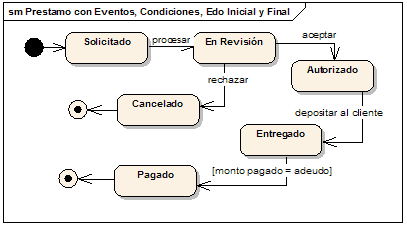
\includegraphics[width=.7\textwidth]{images/edoPrestamo}
		\caption{Máquina de estados de un Préstamo.}
		\label{fig:edos-prestamo}
	\end{center}
\end{figure}

\subsubsection{Estados}

\begin{description}
	\item[Estado:] Descripción del estado.
	\item[...] ...
\end{description}


\subsubsection{Acciones}

\begin{description}
	\item[Acción:] Descripción de la acción indicando el Caso de uso involucrado.
	\item[...] ...
\end{description}


%---------------------------------------------------------
\section{Modelo de Procesos AS-IS}

\cdtInstrucciones{En esta seccion describa todos los procesos tal cual son antesd e desarrollar el proyecto.}

En esta sección se describen los procesos a mejorar con el sistema. En la figura~\ref{fig:mapaProc} se muestra el mapa de procesos y se indican los proceso afectados por el sistema.

\begin{figure}[htbp]
	\begin{center}
		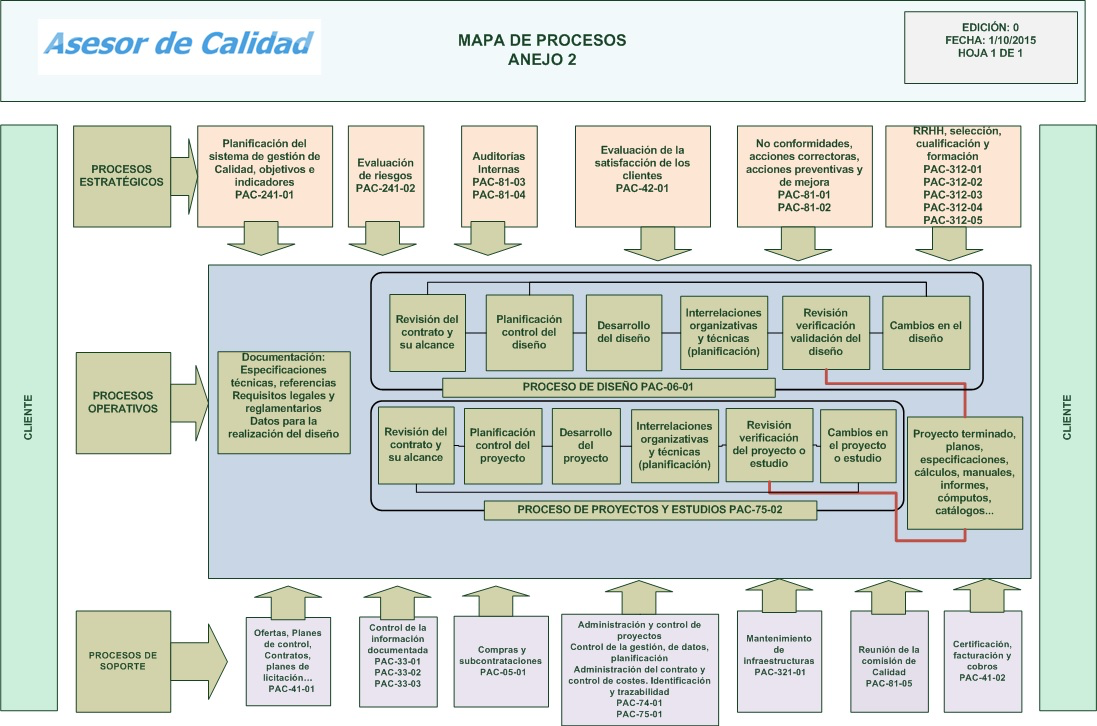
\includegraphics[width=.8\textwidth]{images/mapaProc}
		\caption{Mapa de procesos actual.}
		\label{fig:mapaProc}
	\end{center}
\end{figure}

% !TeX root = ../proyecto.tex




% - - - - - - - - - - - - - - - - - - - - - - - - - - - - 
\subsection{PROC-01 Nombre del proceso}

\begin{figure}[htbp]
	\begin{center}
		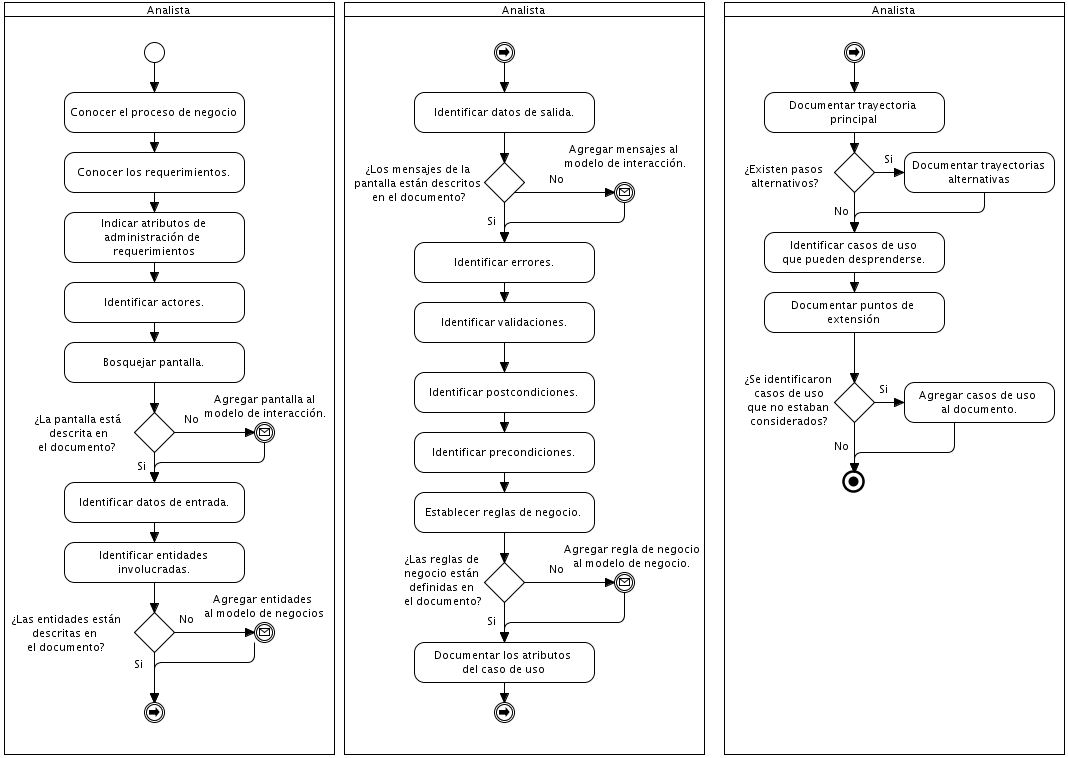
\includegraphics[width=.7\textwidth]{images/proceso1}
		\caption{PROC-01 Proceso de Análisis de requerimientos}
		\label{fig:proceso1}
	\end{center}
\end{figure}

\begin{description}
	\item[Descripción:] Describa el proceso indicando los aspectos relevantes que el diagrama no muestra.
	\item[Entradas:] \cdtEmpty
        \begin{itemize}
			\item Documentos de Procesos.
			\item Reglas de negocio.
			\item Minutas de las reuniones de análisis.
        \end{itemize}
	\item[Salidas:] \cdtEmpty
        \begin{itemize}
			\item Especificación de requerimientos.
			\item Bosquejo de pantallas.
			\item Modelo de base de datos
        \end{itemize}	
    \item[Áreas de oportunidad:] Liste los aspectos que detecta se pueden mejorar con la introducción del sistema o los problemas encontrados.
\end{description}

%\input{proc/proc02.tex}
%\input{proc/proc03.tex}
%\input{proc/proc04.tex}

%---------------------------------------------------------
\section{Modelo de procesos TO-BE}

\cdtInstrucciones{En esta seccion describa todos los procesos modificados una vez que se adopte el sistema.}

Los nuevos procesos se presentan en esta sección, el mapa de procesos de la figura~\ref{fig:mapaProcNvo} se muestra el mapa de procesos actualizado.

\begin{figure}[htbp]
	\begin{center}
		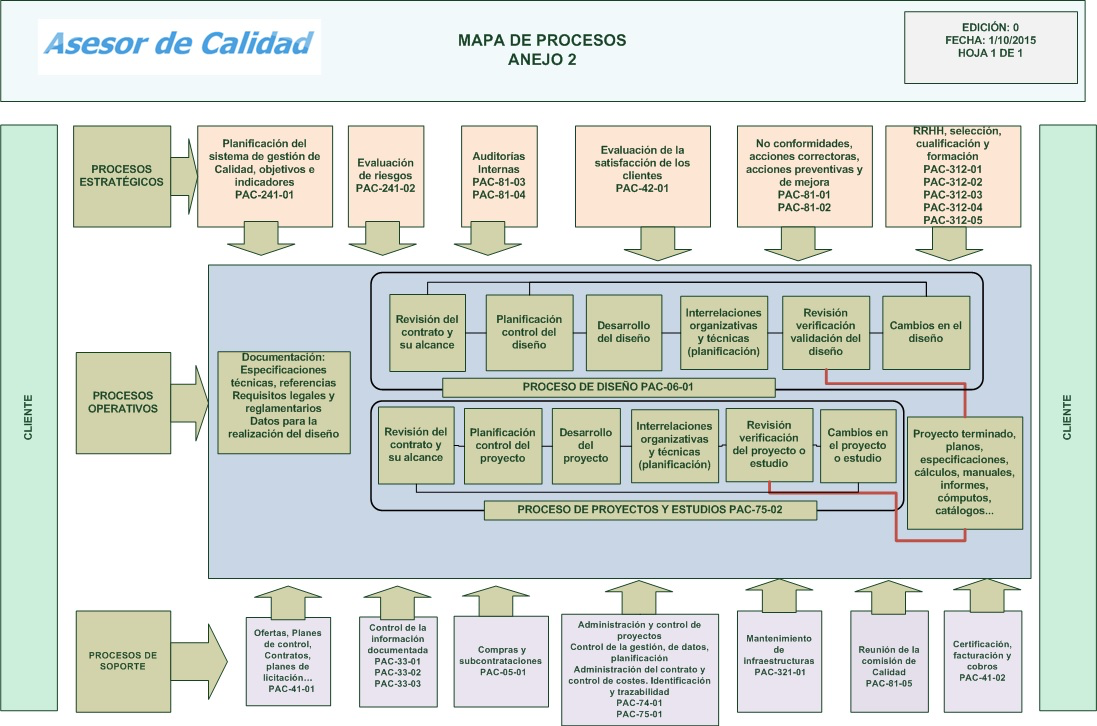
\includegraphics[width=.8\textwidth]{images/mapaProc}
		\caption{Mapa de procesos actualizado}
		\label{fig:mapaProcNvo}
	\end{center}
\end{figure}


% - - - - - - - - - - - - - - - - - - - - - - - - - - - - 
\subsection{PROCM-01 ...}

\begin{figure}[htbp]
	\begin{center}
		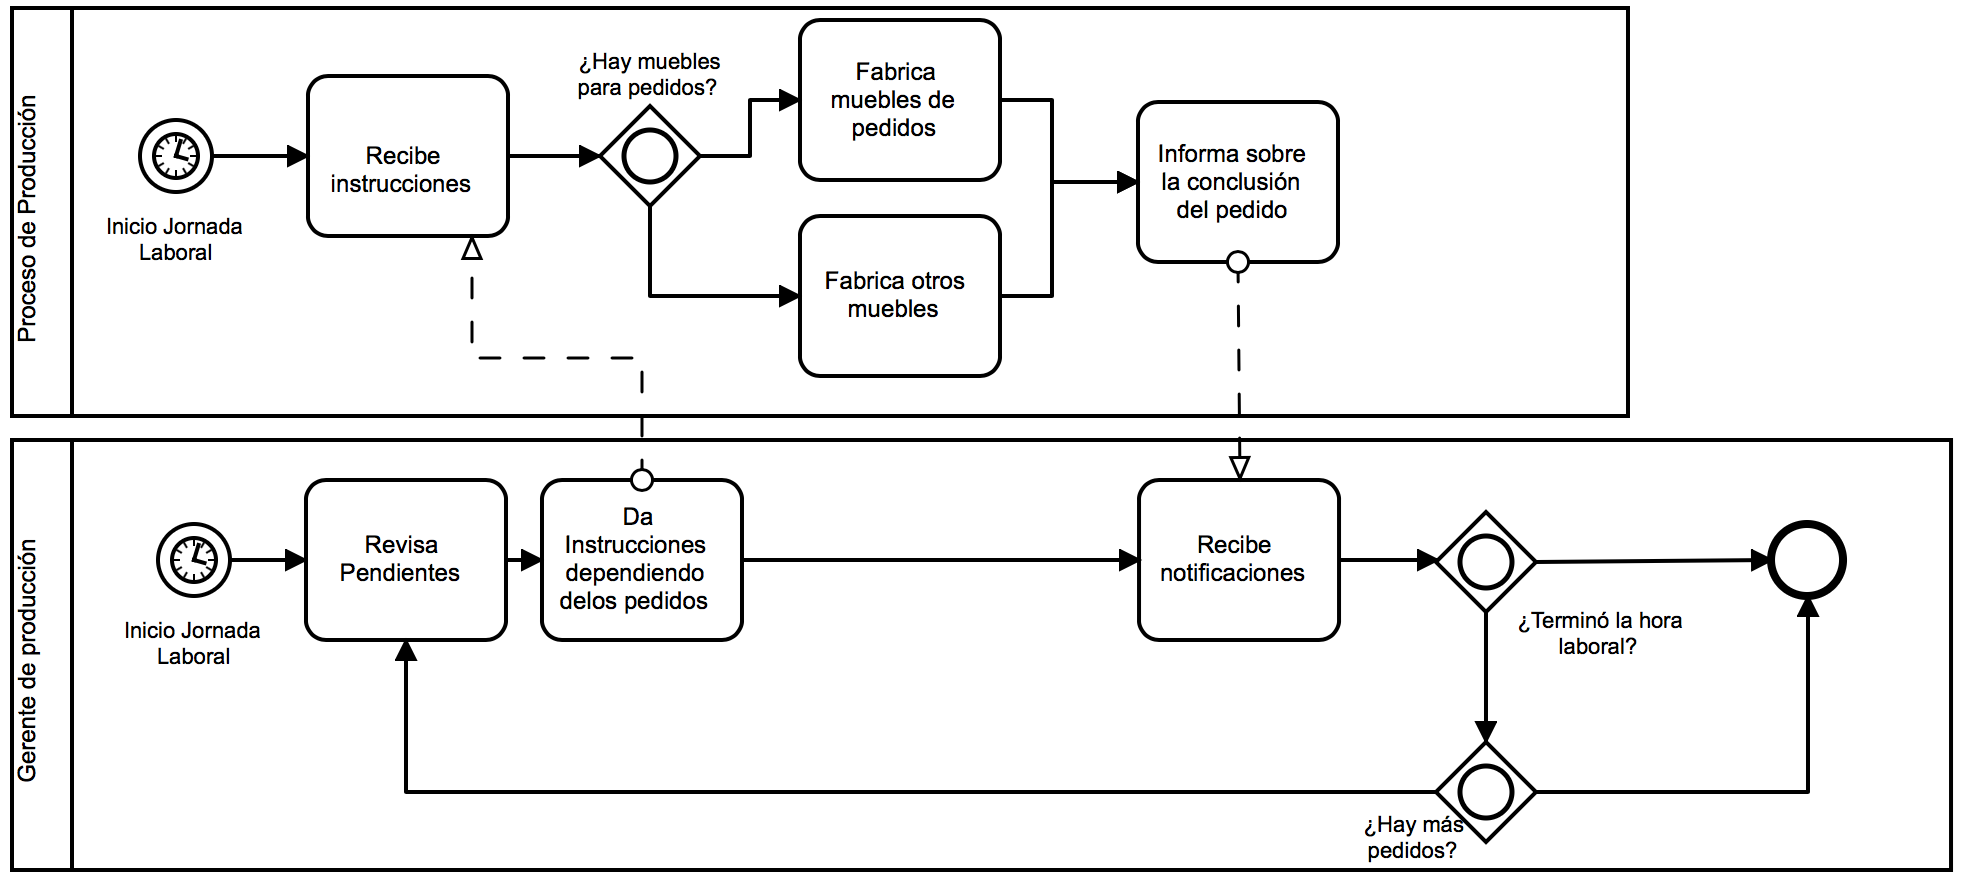
\includegraphics[width=.8\textwidth]{images/proceso3}
		\caption{PROCM-01 Nombre del proceso}
		\label{fig:proceso3}
	\end{center}
\end{figure}

\begin{description}
	\item[Descripción:] ...
	\item[Entradas:] \cdtEmpty
        \begin{itemize}
			\item ...
        \end{itemize}
	\item[Salidas:] \cdtEmpty
        \begin{itemize}
			\item ...
        \end{itemize}	
    \item[Mejoras esperadas:] Liste las mejoras que espera obtener tras la implementación del sistema.
    \item[Reglas de negocio:] \hyperlink{BR05}{BR05}, \hyperlink{BR8}{BR8}.
    \item[Casos de uso:] \hyperlink{CU3.4}{CU 3.4 Login}, \hyperlink{CU 4.3}{ CU 4.3 Consultar productos}.
\end{description}

%\input{proc/proc-m02.tex}
%\input{proc/proc-m03.tex}
%\input{proc/proc-m04.tex}

